\documentclass[xcolor={usenames,dvipsnames}]{beamer}
\usepackage[unilu,en]{collegeBeamer}
\setbeamertemplate{footline}[frame number]
\usepackage{graphicx}
\usepackage{tikz}
\usetikzlibrary{calc, arrows.meta, positioning, shapes.geometric, fit, backgrounds, decorations.pathreplacing}
\usepackage{listings}
\usepackage{fontawesome5}
\usepackage{hyperref}

% Code listing style
\lstset{
    basicstyle=\ttfamily\scriptsize,
    breaklines=true,
    frame=single,
    backgroundcolor=\color{gray!10}
}

% meta-data
\title{Pulse of Engagement}
\subtitle{Visual Analytics for Economic Health in Engagement, OH\\VAST Challenge 2022 -- Challenge 3}
\author{Thomas Gantz \and Michal Sterzel \and Jan Marxen}
\date{December 2025}
\themecolor{50,50,50}

% document body
\begin{document}

% Custom title page with Ohio map
\begin{frame}[plain]
    \centering
    \vspace{0.3cm}
    {\Huge\bfseries Pulse of Engagement}\\[0.25cm]
    {\large Visual Analytics for Economic Health in Engagement, OH}\\[0.1cm]
    {\small VAST Challenge 2022 -- Challenge 3}\\[0.4cm]
    {\normalsize Thomas Gantz \quad Michal Sterzel \quad Jan Marxen}\\[0.2cm]
    {\small December 2025}\\[0.3cm]
    \includegraphics[width=0.35\textwidth]{img/ohio-map-on-white-background-free-vector.jpg}
\end{frame}

% ==============================================================================
\section{Introduction}
% ==============================================================================

\begin{frame}{VAST Challenge 2022 -- Challenge 3}
    \begin{columns}
        \begin{column}{0.55\textwidth}
            \textbf{The Challenge}
            \begin{itemize}
                \item Analyze economic health of a fictional city
                \item Dataset: $\sim$120 million data points
                \item 15 months of 5-minute granularity data
            \end{itemize}
            
            \vspace{10pt}
            \textbf{Three Questions}
            \begin{enumerate}
                \item Business Prosperity
                \item Resident Financial Health
                \item Employer Health \& Turnover
            \end{enumerate}
        \end{column}
        \begin{column}{0.42\textwidth}
            \centering
            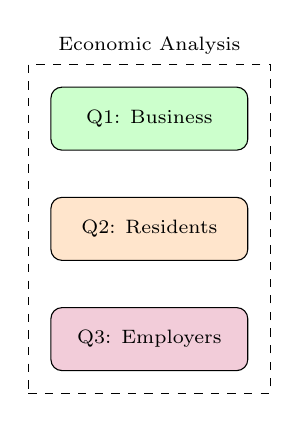
\begin{tikzpicture}[
                scale=0.7,
                box/.style={rectangle, draw, rounded corners, fill=blue!20, minimum width=2.5cm, minimum height=0.8cm, font=\scriptsize, align=center}
            ]
                \node[box, fill=green!20] (q1) at (0,2) {Q1: Business};
                \node[box, fill=orange!20] (q2) at (0,0) {Q2: Residents};
                \node[box, fill=purple!20] (q3) at (0,-2) {Q3: Employers};
                
                \node[rectangle, draw, dashed, fit=(q1)(q2)(q3), inner sep=8pt, label=above:{\scriptsize Economic Analysis}] {};
            \end{tikzpicture}
        \end{column}
    \end{columns}
\end{frame}

\begin{frame}{Our Solution: Pulse of Engagement}
    \centering
    \vspace{5pt}
    
    % TODO: Replace with actual screenshot of the main dashboard
    \fbox{\parbox{0.85\textwidth}{\centering\vspace{2cm}\textbf{[SCREENSHOT: Main Dashboard Overview]}\\\small Show the tabbed interface with all three question areas\vspace{2cm}}}
    
    \vspace{10pt}
    \small
    Interactive web application built with \textbf{React + D3.js} frontend and \textbf{Python Flask} backend
\end{frame}

% ==============================================================================
\section{Question 1: Business Prosperity}
% ==============================================================================

\begin{frame}{\faStore\ Dashboard Overview}
    \centering
    \includegraphics[height=0.92\textheight]{img/businesses_explanation1.png}
\end{frame}

\begin{frame}{\faChartLine\ Growth Analysis}
    \centering
    \includegraphics[height=0.75\textheight]{img/businesses_explanation2.png}
    
    \vspace{8pt}
    \fbox{\parbox{0.9\textwidth}{\small\centering
        \faLightbulb\ \textbf{Key Insight:} Revenue drops in April $\cdot$ Business health is heterogeneous:\\
        $\sim$1/3 growth \textcolor{green!60!black}{\faArrowUp} \quad $\sim$1/3 slight decline \textcolor{orange}{\faArrowDown} \quad $\sim$1/3 significant decline \textcolor{red!70!black}{\faArrowDown}
    }}
\end{frame}

\begin{frame}{\faChartPie\ Market Concentration}
    \centering
    \includegraphics[height=0.75\textheight]{img/businesses_explanation3.png}
    
    \vspace{8pt}
    \fbox{\parbox{0.85\textwidth}{\small\centering
        \faLightbulb\ \textbf{Key Insight:} Two pubs capture 20\% of total spending $\cdot$ Pubs dominate restaurants
    }}
\end{frame}

\begin{frame}{\faClock\ Temporal Trends}
    \begin{columns}[T]
        \begin{column}{0.48\textwidth}
            \centering
            \includegraphics[width=0.85\textwidth]{img/businesses_trend.png}\\[2pt]
        \end{column}
        \begin{column}{0.48\textwidth}
            \centering
            \includegraphics[width=0.85\textwidth]{img/businesses_weekends.png}\\[2pt]
        \end{column}
    \end{columns}
    
    \vspace{8pt}
    \hspace{1cm}\fbox{\parbox{0.85\textwidth}{\small\centering
        \faLightbulb\ \textbf{Key Insight:} Weekend oscillation distinguishes cyclical from structural decline
    }}
\end{frame}

\begin{frame}{\faUser\ Individual Customer Patterns}
    \begin{columns}[T]
        \begin{column}{0.48\textwidth}
            \centering
            \includegraphics[width=0.85\textwidth]{img/businesses_customer1.png}\\[3pt]
        \end{column}
        \begin{column}{0.48\textwidth}
            \centering
            \includegraphics[width=0.85\textwidth]{img/businesses_customer2.png}\\[3pt]
        \end{column}
    \end{columns}
    
    \vspace{8pt}
    \hspace{1cm}\fbox{\parbox{0.85\textwidth}{\small
        \faLightbulb\ \textbf{Micro-level signals:}
        \faHeart\ R\#896: 26\% share $\cdot$
        \faRocket\ P\#894: +27.7\% growth $\cdot$
        \faBan\ R\#1349: abandoned
    }}
\end{frame}

\begin{frame}{\faClipboardList\ Key Findings}
    \begin{columns}[T]
        \begin{column}{0.48\textwidth}
            {\large \textcolor{green!60!black}{\faThumbsUp\ Prosperous}}
            \begin{itemize}
                \item[\textcolor{green!60!black}{\faCheck}] Pubs outperform restaurants
                \item[\textcolor{green!60!black}{\faCheck}] P\#1342, P\#1344 dominate market
            \end{itemize}
        \end{column}
        \begin{column}{0.48\textwidth}
            {\large \textcolor{red!70!black}{\faThumbsDown\ Struggling}}
            \begin{itemize}
                \item[\textcolor{red!70!black}{\faTimes}] Top performers decline in H2
                \item[\textcolor{red!70!black}{\faTimes}] $\sim$1/3 show substantial drops
            \end{itemize}
        \end{column}
    \end{columns}
    
    \vspace{15pt}
    \centering
    \fcolorbox{red!50!black}{red!5}{\parbox{0.85\textwidth}{\centering
        \faExclamationTriangle\ \textbf{Overall:} Aggregate spending declining over 15 months
    }}
\end{frame}

\begin{frame}{\faPencilRuler\ Design Rationale}
    \textbf{\faLayerGroup\ Visualization Progression}
    \begin{enumerate}
        \item[\faEye] \textbf{Overview} $\rightarrow$ establish baseline context
        \item[\faFilter] \textbf{Temporal filtering} $\rightarrow$ identify patterns over time
        \item[\faSearchPlus] \textbf{Individual detail} $\rightarrow$ surface micro-level signals
    \end{enumerate}
    
    \vspace{12pt}
    \textbf{\faCogs\ Key Design Decisions}
    \begin{itemize}
        \item[\faLink] \textbf{Coordinated views:} hover-linking for cross-chart exploration
        \item[\faBalanceScale] \textbf{Split-period comparison:} quantifies growth directly
        \item[\faSlidersH] \textbf{Global filters:} all-to-all, one-to-all, one-to-one analysis
        \item[\faChartBar] \textbf{Dual metrics:} visits and spending reveal correlation
    \end{itemize}
\end{frame}

% ==============================================================================
\section{Question 2: Resident Financial Health}
% ==============================================================================

\begin{frame}{Q2: Analysis Approach}
    \vspace{-5pt}
    \textbf{Three Complementary Lenses}
    \vspace{5pt}
    \begin{columns}[T]
        \begin{column}{0.32\textwidth}
            \centering
            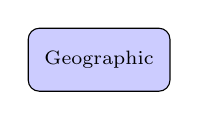
\begin{tikzpicture}
                \node[rectangle, draw, rounded corners, fill=blue!20, minimum width=1.8cm, minimum height=0.8cm, font=\scriptsize, align=center] {Geographic};
            \end{tikzpicture}
            \footnotesize
            \begin{itemize}\setlength{\itemsep}{1pt}
                \item Building heatmap
                \item Savings by location
                \item Identify red zones
            \end{itemize}
        \end{column}
        \begin{column}{0.32\textwidth}
            \centering
            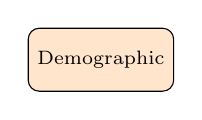
\begin{tikzpicture}
                \node[rectangle, draw, rounded corners, fill=orange!20, minimum width=1.8cm, minimum height=0.8cm, font=\scriptsize, align=center] {Demographic};
            \end{tikzpicture}
            \footnotesize
            \begin{itemize}\setlength{\itemsep}{1pt}
                \item Wage vs. cost
                \item K-Means clustering
                \item Savings drivers
            \end{itemize}
        \end{column}
        \begin{column}{0.32\textwidth}
            \centering
            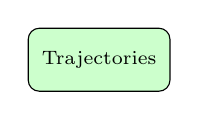
\begin{tikzpicture}
                \node[rectangle, draw, rounded corners, fill=green!20, minimum width=1.8cm, minimum height=0.8cm, font=\scriptsize, align=center] {Trajectories};
            \end{tikzpicture}
            \footnotesize
            \begin{itemize}\setlength{\itemsep}{1pt}
                \item Income vs. expenses
                \item Inequality trends
                \item Time evolution
            \end{itemize}
        \end{column}
    \end{columns}
\end{frame}

\begin{frame}{Geographic Financial Health}
    \begin{columns}[T]
        \begin{column}{0.45\textwidth}
            \textbf{Building-Level Heatmap}
            \footnotesize
            \begin{itemize}\setlength{\itemsep}{2pt}
                \item Colors by average savings rate
                \item Red: break-even or negative
                \item Yellow: moderate savings
                \item Green: high savings
            \end{itemize}
            
            \vspace{6pt}
            \textbf{Insights}
            \begin{itemize}\setlength{\itemsep}{2pt}
                \item ``Red pockets'' persist over time
                \item Chronic, not worsening, conditions
                \item Mini-clusters suggest local stressors
            \end{itemize}
        \end{column}
        \begin{column}{0.52\textwidth}
            \centering
            \includegraphics[width=\textwidth,height=0.80\textheight,keepaspectratio]{img/geog_fin_health.png}
        \end{column}
    \end{columns}
\end{frame}

\begin{frame}{Resident Profile: Affluent Achievers}
    \begin{columns}[T]
        \begin{column}{0.32\textwidth}
            \scriptsize
            \vspace{0pt}
            {\large \color{red!70!black}\bfseries Affluent Achievers}
            
            \vspace{5pt}
            \textbf{Main Characteristics}
            \begin{itemize}\setlength{\itemsep}{2pt}
                \item High income levels
                \item Predominantly graduate education
                \item Significant financial buffer
            \end{itemize}
            
            \vspace{8pt}
            \textbf{Median Statistics (Apr 2022)}
            \begin{itemize}\setlength{\itemsep}{2pt}
                \item \textbf{Income:} \$5{,}756
                \item \textbf{Cost:} \$1{,}419
                \item \textbf{Savings:} 76.6\%
            \end{itemize}
        \end{column}
        \begin{column}{0.66\textwidth}
            \centering
            \includegraphics[width=\textwidth,height=0.46\textheight,keepaspectratio]{img/affluent_PCP.png}\\[1pt]
            \includegraphics[width=\textwidth,height=0.46\textheight,keepaspectratio]{img/affluent_scatter.png}
        \end{column}
    \end{columns}
\end{frame}

\begin{frame}{Resident Profile: Stretched Households}
    \begin{columns}[T]
        \begin{column}{0.32\textwidth}
            \scriptsize
            \vspace{0pt}
            {\large \color{blue!70!black}\bfseries Stretched Households}
            
            \vspace{5pt}
            \textbf{Main Characteristics}
            \begin{itemize}\setlength{\itemsep}{2pt}
                \item Larger households, often with children
                \item Tightest budget constraints
                \item "Living Gap" pressure is highest here
            \end{itemize}
            
            \vspace{8pt}
            \textbf{Median Statistics (Apr 2022)}
            \begin{itemize}\setlength{\itemsep}{2pt}
                \item \textbf{Income:} \$2{,}869
                \item \textbf{Cost:} \$1{,}405
                \item \textbf{Savings:} 51.0\%
            \end{itemize}
        \end{column}
        \begin{column}{0.66\textwidth}
            \centering
            \includegraphics[width=\textwidth,height=0.46\textheight,keepaspectratio]{img/stretched_PCP.png}\\[1pt]
            \includegraphics[width=\textwidth,height=0.46\textheight,keepaspectratio]{img/stretched_scatter.png}
        \end{column}
    \end{columns}
\end{frame}

\begin{frame}{Resident Profile: Lean Savers}
    \begin{columns}[T]
        \begin{column}{0.32\textwidth}
            \scriptsize
            \vspace{0pt}
            {\large \color{orange!70!black}\bfseries Lean Savers}
            
            \vspace{5pt}
            \textbf{Main Characteristics}
            \begin{itemize}\setlength{\itemsep}{2pt}
                \item Smaller households
                \item Typically without children
                \item Moderate income, but lower costs than families
            \end{itemize}
            
            \vspace{8pt}
            \textbf{Median Statistics (Apr 2022)}
            \begin{itemize}\setlength{\itemsep}{2pt}
                \item \textbf{Income:} \$3{,}352
                \item \textbf{Cost:} \$1{,}586
                \item \textbf{Savings:} 54.5\%
            \end{itemize}
        \end{column}
        \begin{column}{0.66\textwidth}
            \centering
            \includegraphics[width=\textwidth,height=0.46\textheight,keepaspectratio]{img/lean_PCP.png}\\[1pt]
            \includegraphics[width=\textwidth,height=0.46\textheight,keepaspectratio]{img/lean_scatter.png}
        \end{column}
    \end{columns}
\end{frame}

\begin{frame}{What Drives Savings?}
    \begin{columns}[T]
        \begin{column}{0.35\textwidth}
            \textbf{Demographic Drivers}
            \vspace{5pt}
            
            \footnotesize
            \textbf{Savings rate predictors ($\Delta R^2$)}
            \scriptsize
            \begin{itemize}\setlength{\itemsep}{1pt}
                \item Cost of living (0.828)
                \item Income (0.408)
                \item Household size (0.376)
                \item Has kids (0.127)
            \end{itemize}

            \vspace{10pt}
            \footnotesize
            \textbf{Cluster separators ($\eta^2$)}
            \scriptsize
            \begin{itemize}\setlength{\itemsep}{1pt}
                \item Has kids (83.1\%)
                \item Graduate education (72.0\%)
                \item Household size (61.9\%)
                \item Income (38.0\%)
            \end{itemize}
        \end{column}
        \begin{column}{0.65\textwidth}
            \centering
            \vspace{-10pt}
            \includegraphics[width=\textwidth,height=0.85\textheight,keepaspectratio]{img/scatter.png}
        \end{column}
    \end{columns}
\end{frame}

\begin{frame}{Inequalities Over Time}
    \vspace{-8pt}
    
    % Wide Gini plot at top
    \begin{center}
        \includegraphics[width=0.95\textwidth,height=0.48\textheight,keepaspectratio]{img/gini_inequality.png}
    \end{center}
    
    \vspace{8pt}
    
    % Text content below in two columns
    \begin{columns}[T]
        \begin{column}{0.48\textwidth}
            \textbf{Inequality Trends}
            \footnotesize
            \begin{itemize}\setlength{\itemsep}{1pt}
                \item Gini coefficient tracks disparity
                \item Income inequality stable over time
                \item Savings inequality slightly higher
            \end{itemize}
        \end{column}
    \end{columns}
\end{frame}

\begin{frame}{Expense Dynamics Over Time}
    \vspace{-8pt}
    
    % Wide financial trajectories plot
    \begin{center}
        \includegraphics[width=\textwidth,height=1.0\textheight,keepaspectratio]{img/financial_flow.png}
    \end{center}

\end{frame}

% ==============================================================================
\section{Question 3: Employer Health}
% ==============================================================================

\begin{frame}{Q3: Employer Health \& Turnover}
    \centering
    \vspace{1cm}
    
    {\Large \textbf{[PLACEHOLDER FOR MICHAL]}}
    
    \vspace{1cm}
    
    \begin{itemize}
        \item Employment patterns across the city
        \item Turnover rate analysis
        \item High/low turnover areas
    \end{itemize}
    
    \vspace{1cm}
    
    % TODO: Add screenshots of employer visualizations
    \fbox{\parbox{0.7\textwidth}{\centering\vspace{1.5cm}\textbf{[SCREENSHOT: Employer Visualizations]}\vspace{1.5cm}}}
\end{frame}

\begin{frame}{Q3: Key Findings}
    \centering
    \vspace{1cm}
    
    {\Large \textbf{[PLACEHOLDER FOR MICHAL]}}
    
    \vspace{1cm}
    
    \begin{columns}
        \begin{column}{0.48\textwidth}
            \textbf{Healthy Employers}
            \begin{itemize}
                \item [To be filled by teammate]
            \end{itemize}
        \end{column}
        \begin{column}{0.48\textwidth}
            \textbf{High Turnover Areas}
            \begin{itemize}
                \item [To be filled by teammate]
            \end{itemize}
        \end{column}
    \end{columns}
\end{frame}

% ==============================================================================
\section{Design Decisions}
% ==============================================================================

\begin{frame}{Tech Stack}
    \begin{columns}
        \begin{column}{0.48\textwidth}
            \textbf{Frontend}
            \begin{itemize}
                \item \textbf{React 18} -- Component architecture
                \item \textbf{D3.js v7} -- Visualization rendering
                \item \textbf{TailwindCSS} -- Styling
                \item \textbf{Axios} -- API communication
            \end{itemize}
            
            \vspace{8pt}
            \textbf{Infrastructure}
            \begin{itemize}
                \item \textbf{Docker Compose} -- Orchestration
                \item \textbf{Nginx} -- Reverse proxy
            \end{itemize}
        \end{column}
        \begin{column}{0.48\textwidth}
            \textbf{Backend}
            \begin{itemize}
                \item \textbf{Python 3.11} -- Core language
                \item \textbf{Flask} -- REST API
                \item \textbf{Pandas/NumPy} -- Data processing
                \item \textbf{Scikit-learn} -- K-Means clustering
                \item \textbf{Pytest} -- Testing
            \end{itemize}
        \end{column}
    \end{columns}
    
    \vspace{12pt}
    \centering
    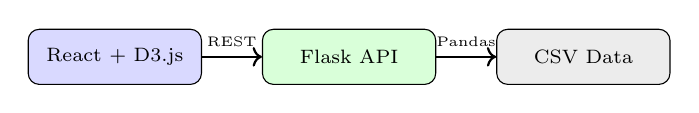
\begin{tikzpicture}[scale=0.85]
        \node[rectangle, draw, rounded corners, fill=blue!15, minimum width=2.2cm, minimum height=0.7cm, font=\scriptsize] (fe) at (-3.5,0) {React + D3.js};
        \node[rectangle, draw, rounded corners, fill=green!15, minimum width=2.2cm, minimum height=0.7cm, font=\scriptsize] (be) at (0,0) {Flask API};
        \node[rectangle, draw, rounded corners, fill=gray!15, minimum width=2.2cm, minimum height=0.7cm, font=\scriptsize] (data) at (3.5,0) {CSV Data};
        
        \draw[->, thick] (fe) -- node[above, font=\tiny] {REST} (be);
        \draw[->, thick] (be) -- node[above, font=\tiny] {Pandas} (data);
    \end{tikzpicture}
\end{frame}


% ==============================================================================
\section{Team Organization}
% ==============================================================================

\begin{frame}{Work Organization}
    \begin{columns}
        \begin{column}{0.55\textwidth}
            \textbf{Division of Work}
            \begin{itemize}
                \item One question per team member
                \item Shared infrastructure setup
                \item Code reviews via Git
            \end{itemize}
            
            \vspace{10pt}
            \begin{tabular}{ll}
                	\textbf{Thomas} & Q1: Business Prosperity \\
                	\textbf{Jan} & Q2: Resident Financial Health \\
                	\textbf{Michal} & Q3: Employer Health \\
            \end{tabular}
        \end{column}
        \begin{column}{0.42\textwidth}
            \textbf{Shared Components}
            \begin{itemize}
                \item Docker infrastructure
                \item API structure
                \item Test framework
            \end{itemize}
            
            \vspace{8pt}
            \textbf{Communication}
            \begin{itemize}
                \item Regular syncs and feedback
                \item Clear API contracts
            \end{itemize}
        \end{column}
    \end{columns}
\end{frame}



% ==============================================================================
\section{Lessons Learned}
% ==============================================================================

\begin{frame}{Lessons Learned}
    \begin{columns}
        \begin{column}{0.48\textwidth}
            \textbf{What Worked Well}
            \begin{itemize}
                \item \textcolor{green!60!black}{\faCheck} Docker for reproducibility
                \item \textcolor{green!60!black}{\faCheck} Clear question separation
                \item \textcolor{green!60!black}{\faCheck} Caching for large datasets
                \item \textcolor{green!60!black}{\faCheck} Test-driven development
            \end{itemize}
        \end{column}
        \begin{column}{0.48\textwidth}
            \textbf{Challenges}
            \begin{itemize}
                \item \textcolor{red!60!black}{\faTimes} TODO
            \end{itemize}
            
            \vspace{8pt}
            \textbf{Would Do Differently}
            \begin{itemize}
                \item TODO
            \end{itemize}
        \end{column}
    \end{columns}
\end{frame}

% ==============================================================================
\section{}
% ==============================================================================

\begin{frame}{}
    \centering
    \vspace{1.5cm}
    {\Huge \textbf{Thank You!}}
    
    \vspace{1cm}
    {\large Questions?}
    
    \vspace{1cm}
    \begin{tabular}{ccc}
        Thomas Gantz & Jan Marxen & Michal Sterzel \\
        \scriptsize Q1: Business & \scriptsize Q2: Residents & \scriptsize Q3: Employers \\
    \end{tabular}
    
    \vspace{0.8cm}
    \small
    \faGithub\ \url{github.com/janmarxen/VAST-challenge}
    
    \vspace{0.5cm}
    \scriptsize
    Data Visualization -- EUMaster4HPC -- December 2025
\end{frame}

\end{document}
